\chapter{Creating Variables in Opus}
\label{chap:creating-variables}

As described in the previous chapter (Chapter \ref{chap:data-in-opus}),
datasets contain primary and computed attributes.  Computed attributes
are defined as Opus variables.  In many cases, these variables can be
defined in a domain-specific programming language (called Tekoa).  When
this can be done, it is much simpler than defining them in Python itself.
The syntax of the Tekoa language is described in the next section.

\section{Opus Expressions}
\label{sec:expressions}
\index{expressions}

Opus uses Python and Numpy to create variables to be used in models.  These are often coded in Python modules as
described in the preceding section.  However, in order to make the use of variables simpler for users to access, a new
\emph{expression language} has been created for Opus
that allows variables to be defined with a relatively simple and concise syntax.  In fact, at this point, many of the variables that
have been previously implemented as modules could be replaces by simpler one-line expressions using this language.

The syntax consists of using Numpy operations and methods, operating on Opus variables and primary data.  All of the Numpy operators are available, and work in the same way for expressions, including \verb#+ -  * / **#, where ** is an exponential function: a**3 returns a to the power of 3.

Expressions allow an \verb#alias#, or name, to be assigned to the expression, in order to use it by this reference in a model specification or indicator function.  The standard syntax in Opus uses short names, with lower case letters.  If two or more words are used in a name, we usually separate the components with an underscore to make the name more readable.  Some examples will illustrate key aspects of the expression syntax:

\begin{itemize}

\item \code{hwy\_300 = gridcell.distance\_to\_highway<300} would generate a dummy variable equal to 1 for gridcells that have an attribute value of distance to highway less than 300 meters.  Note that in this case we are operating on a \verb#primary attribute# of gridcells, which means that it is part of the data that we initially load into the model, as opposed to data we compute within the model.

\item \code{ln\_pop = ln(urbansim.gridcell.population} would be used to compute the log of an existing variable, population, which is in the urbansim package and applies to the gridcell dataset.

\item \code{pop\_emp\_ratio = urbansim.gridcell.population / urbansim.gridcell.number\_of\_jobs} would compute the ratio of population to employment, using variables stored in the urbansim package, associated with the gridcell dataset.  

\end{itemize}

Two very useful methods in the expression language are \verb#aggregation# and \verb#disaggregation#.  Aggregation allows an expression to compute a result on one dataset and aggregate the results to assign to another dataset, such as summing the population in households that live in a gridcell.  Using this expression approach, we could replace the long population.py module in the preceding section with the following expression:

\code{population = gridcell.aggregate(household.persons)}

That is quite a lot easier to understand and to code!  We are aggregating to the gridcell dataset, from the household dataset, the number of persons.  However, in the time since the variable in the preceding section was implemented, we have changed the data structure for the gridcell and parcel based models to use buildings.  So now, households and jobs are associated with buildings, and buildings are associated with gridcells (or parcels).  This means that in order to compute the population of a gridcell, we need to first aggregate it to building, and then from building to gridcell.  That is not hard to do, either, by simply adding an intermediated argument to the aggregation function.  There can be multiple levels of intermediates, if needed:

\code{population = gridcell.aggregate(household.persons, intermediates = [building])}

The default method for aggregation is to sum, but there are several other aggregation methods available also:

\squishlist
\item sum
\item mean
\item maximum
\item mininim
\item variance
\item standard\_deviation
\item center\_of\_mass
\squishend

To use any of these functions, we simply add \verb#function = mean# (or another function) in the expression.  Here is an example to determine the average household size per gridcell:

\code{avg\_hhs = gridcell.aggregate(households.persons, intermediates = [building], function = mean)}

The \verb#disaggregate# method for expressions assigns values from one dataset to another, in a one to many relationship.  In other words, it works in the opposite direction from the aggregate method, which is many to one.  An example would be to assign the zonal population density to all households living the zone.  In this example, we use the \verb#population_density# variable in the zone dataset of the urbansim\_parcel package, and assign it to households, which are connected to zones indirectly through buildings and then parcels: household -$>$ building -$>$ parcel -$>$ zone.  So the expression would be:

\code{density = household.disaggregate(urbansim\_parcel.zone.population\_density, intermediates = [building, parcel])}

Note that for both aggregate and disaggregate methods, the first element, preceding the method name, is the name of the dataset to which the result should be assigned.  zone.aggregate... should generate some result and assign it to zone, whereas gridcell.disaggregate... should assign some value from a larger geography to the gridcell dataset.

A list of expressions can be stores in an \verb#aliases.py# file within a package and dataset directory.  This provides an efficient means to organize and store many expressions in a single location.  Below are some of the aliases in the urbansim\_parcel/parcel/aliases.py module that demonstrate some of the expressions in actual use in the model system.\\

%\begin{lstlisting}
"used_land_area = (parcel.aggregate(building.land_area, function=sum)).astype(int32)",
"vacant_land_area = parcel.parcel_sqft - urbansim_parcel.parcel.used_land_area",
"unit_name = parcel.disaggregate(land_use_type.unit_name)",
"building_sqft = (parcel.aggregate(urbansim_parcel.building.building_sqft)).astype(int32)",
"building_sqft_per_unit = safe_array_divide(urbansim_parcel.parcel.building_sqft, urbansim_parcel.parcel.residential_units)",
"residential_units = (parcel.aggregate(building.residential_units)).astype(int32)",       
"parcel_sqft_per_unit = safe_array_divide( parcel.parcel_sqft, (urbansim_parcel.parcel.residential_units).astype(float32) )",
"unit_price = safe_array_divide(parcel.land_value + urbansim_parcel.parcel.improvement_value, urbansim_parcel.parcel.existing_units)",
"demolition_cost = (parcel.aggregate(urbansim_parcel.building.demolition_cost)).astype(int32)",
"improvement_value = (parcel.aggregate(building.improvement_value)).astype(int32)",
"total_value_per_sqft = safe_array_divide(parcel.land_value + urbansim_parcel.parcel.improvement_value, parcel.parcel_sqft)",
"number_of_jobs = parcel.aggregate(urbansim_parcel.building.number_of_jobs)",
"employment = parcel.aggregate(urbansim_parcel.building.number_of_jobs)",
"number_of_households = parcel.aggregate(urbansim_parcel.building.number_of_households)",
"population = parcel.aggregate(urbansim_parcel.building.population)",
"travel_time_to_cbd = parcel.disaggregate(gridcell.travel_time_to_cbd)",       
%\end{lstlisting}

\section{Expressions}
\label{sec:urbansim-tutorial-expressions}
\index{expressions}

In many cases variable definitions are simple expressions involving other
variables.  For these cases, Opus provides an \emph{expression language}
that allows them to be defined succinctly, rather than requiring the Opus
user to write new variable definitions in Python.  (The expression language
has been added recently to Opus, and there are many explicitly declared
variables in the existing UrbanSim package that are no longer needed ---
they could be written as expressions instead in the specifications.  We
plan to remove these unneeded variables in the future.)

The syntax of the expression language is that of Python, but the semantics
are somewhat different --- for example, a name like
\code{gridcell.distance_to_cbd} is a reference to the value of that
variable.  (If you just evaluated this in a Python shell you'd get an
error, saying that the \package{gridcell} package didn't have a
\code{distance_to_cbd} attribute.)  Further, expressions are evaluated lazily.

An expression consists of an attribute name, or a function or operation
applied to other expressions.  This definition is recursive, so that a
function or operation can be applied to expressions composed
from other expressions.  For example, here are some legal expressions:

\begin{itemize}

\item \code{urbansim.gridcell.population}
\item \code{ln(urbansim.gridcell.population)+1}

\end{itemize}

\subsection{Variable Names in Expressions}

The attribute names used in an expression can be:

\begin{itemize}
\item a fully-qualified variable name (for an existing variable).  Example:
\code{urbansim.gridcell.population}.

\item a dataset-qualified variable name or primary attribute.
Example: \code{household.income}.
\end{itemize}

The variable names can include arguments (Section
\ref{sec:tutorial-numbersinvariables}).\index{Variable!arguments}\index{arguments to variables}
For example,
\class{is_near_highway_if_threshold_is_2} matches the variable definition
for \class{is_near_SSS_if_threshold_is_DDD}.\footnote{This syntax for
arguments to variables is not ideal --- we hope to replace it with a
more standard syntax in the future.}

\subsection{Unary Functions for Opus Expressions}
\label{sec:functions-for-opus-expressions}

There is a set of unary functions defined to use in expressions, as
follows.  These all operate on numpy arrays.

\begin{description}

\item[\code{clip_to_zero}] Returns the input values with all negative values
   clipped to 0. \index{clip_to_zero}

\item[\code{exp}] Returns an array consisting of $e$ raised to the input 
values.\index{exp}

\item[\code{ln}] Returns an array of natural logarithms.  Input values of 0
result in 0.  (The intent is that this function be used on arrays of
values, where 0 denotes a missing value.  However, be cautious --- as you
approach 0 from the positive side, the result value becomes more and more
negative, and then suddenly returns to 0 at 0.)  \index{ln}

\item[\code{ln_bounded}] Returns an array of natural logarithms. Values
less than 1 result in 0.  \index{ln_bounded}

\item[\code{ln_shifted}] Returns an array of natural logarithms.  The input
  values are shifted by the second argument before taking the log.  (The
  default shift value is 1.)  \index{ln_shifted}

\item[\code{ln_shifted_auto}] If the input values includes values that are
less than or equal to 0, they are shifted so that the minimum of the
shifted values is 1 before taking the log.  Otherwise the log is taken on
the original values.  \index{ln_shifted_auto}

\item[\code{sqrt}] Returns an array of square roots.  Values less than 0
  result in 0. \index{sqrt}

\item[\code{safe_array_divide}] First three arguments are the nominator, denominator and 
a constant. The function returns an array of numerator / denominator for all values where denominator is not 0,
otherwise the constant (default value is 0). An optional fourth argument controls
the type of the resulting array. The default value is 'float32'.
\end{description}

In addition, all of the functions in numpy are available.  To avoid name
collisions, the function name in an expression must include the package
name \code{numpy}.  For example, this expression gives you the reciprocals
of all the values in a variable \code{v}:

\code{numpy.reciprocal(v)}

\subsection{Operators for Opus Expressions}
\index{numpy!operators}

All of the numpy operators can be used in Opus expressions, including
\verb|+ - * / ** |.  Note the numpy semantics for these --- for example,
\verb|*| does elementwise multiplication of two numpy arrays, or with a
scalar argument, scales all the elements in an array,
e.g.\ \code{1.2*household.income}.

\subsection{Aliasing}
\label{sec:aliasing}
\index{aliasing}

A new attribute name can be declared and initialized using an assignment
statement:

\code{lnpop = ln(urbansim.gridcell.population)}

This is treated as an expression, which can occur in the list of
expressions given to \method{compute_variables} or in an \file{aliases.py}
file (see below).  The value of the new alias is returned as the value of
the expression if it's the last item on the list of variables and
expressions.

It is convenient, and often more efficient, to gather all the expressions
and aliases for a particular package and dataset into one place.  The
optional \file{aliases.py} file supports this.  \index{alias.py file}
This file should define a
single variable \code{aliases} to be a list of expressions, each of which
should define an alias.  This file is then placed in the same directory as
variables for that package and dataset.  For example, to define aliases
relevant to \code{urbansim.gridcell}, put an \file{aliases.py} file into
the \file{urbansim.gridcell} directory.  These aliases can then be referred
to using the fully-qualified name of the alias.  When finding a variable
referenced by a fully-qualified name, the system first searches the aliases
file (if present), and then the variable definitions in the appropriate
directory.

As an example, the directory \code{opus_core.test_agent} contains one
variable definition, for the variable \code{income_times_2}.  (This
directory and variable are used for unit tests for \package{opus_core}.)
The file \file{aliases.py} in that same directory contains the following:

\begin{verbatim}
aliases = [
    'income_times_5 = 5*opus_core.test_agent.income',
    'income_times_10 = 5*opus_core.test_agent.income_times_2'
    ]
\end{verbatim}

The first alias refers to a primary attribute (\code{test_agent.income}),
and the second to the variable.  These aliases can then be referred to
using a fully-qualified name, in exactly the same way as a variable,
for example

\code{opus_core.test_agent.income_times_5}.  

See the unit tests in
\file{opus_core.variables.expression_tests.aliases_file} for examples of
using these aliases.

\subsection{Casting the Value of an Expression}
\index{casting}

Normally the value of a variable defined by an expressions will be a
\code{float64} (this is a numpy type).  For large datasets this may use too
much space.  You can cast the result of any expression to a different type
using the numpy \code{astype} method.  For example, the alias defined by
this expression will be of type \code{float32}:

\begin{verbatim}
lnpop = ( ln(urbansim.gridcell.population) ).astype(float32)
\end{verbatim}

The following numpy types can be used as the argument to the \code{astype}
method: \code{bool8}, \code{int8}, \code{uint8}, \code{int16},
\code{uint16}, \code{int32}, \code{uint32}, \code{int64}, \code{uint64}
\code{float32}, \code{float64}, \code{complex64}, \code{complex128}, and
\code{longlong}.
 
\subsection{Interaction Sets}
\index{interaction sets}

If you access an attribute of a component of an interaction set in the
context of that interaction set, the result is converted into a 2-d array
and returned.  These 2-d arrays can then be multiplied, divided, compared,
and so forth, using the numpy functions and operators.  For example,
suppose we have an interaction set \file{household_x_gridcell}.  The
component \file{household} set has an attribute \verb|income| with values
\verb|[100, 200, 300]|.  (These numbers are just to explain the concepts
--- obviously they aren't realistic incomes.)  The \file{gridcell}
component has an attribute \verb|cost| with values \verb|[1000, 1200]|.
Then evaluating

\begin{verbatim}
household_x_gridcell.compute_variables('urbansim.household.income')
\end{verbatim}

will return a 2-d array

\begin{verbatim}
[ [100, 100],
  [200, 200],
  [300, 300] ]
\end{verbatim}

and

\begin{verbatim}
household_x_gridcell.compute_variables('urbansim.gridcell.cost')
\end{verbatim}

returns

\begin{verbatim}
[ [1000, 1200],
  [1000, 1200],
  [1000, 1200] ]
\end{verbatim}

Then
\begin{verbatim}
household_x_gridcell.compute_variables(
            'urbansim.gridcell.cost*urbansim.household.income')
\end{verbatim}

evaluates to
\begin{verbatim}
[ [100000, 120000],
  [200000, 240000],
  [300000, 360000] ]
\end{verbatim}

Both the arguments to the operation and the result can be used in more
complex expressions.  For example, if we wanted to give everyone
a \$5000 income boost, and also scale the result, this could be done using
\verb|(household.income+5000)*gridcell.cost * 1.2|.

As another example, the model specification from
page~\pageref{page:iv-spec} can be modified by using an expression for the
interaction and taking its log: \variablesindex \coefficientsindex

\begin{verbatim}
>>> specification = EquationSpecification(
      variables=("gridcell.cost",
         "ln(urbansim.gridcell.cost*urbansim.household.income)"),
      coefficients=("costcoef", "cti_coef"))
\end{verbatim}


\subsection{Aggregation and Disaggregation}
\label{sec:aggregation}
\index{aggregation} \index{disaggregation}

The methods \class{aggregate} and \class{disaggregate} are used to
aggregate and disaggregate variable values over two or more datasets.  
\index{aggregate} \index{disaggregate} The \class{aggregate} method associates
information from one dataset to another along a many-to-one relationship, while
the \class{disaggregate} method does the same along a one-to-many relationship. Some
examples are:

\begin{itemize}
\item \code{zone.aggregate(gridcell.population)}

\item \code{zone.aggregate(2.5*gridcell.population)}

\item \code{zone.aggregate(urbansim.gridcell.population)}

\item \code{neighborhood.aggregate(gridcell.population, 
  intermediates=[zone,faz])}

\item \code{neighborhood.aggregate(gridcell.population, 
  intermediates=[zone, faz], function=mean)}

\item \code{zone.aggregate(gridcell.population, function=mean)}

\item \code{region.aggregate_all(zone.my_variable)}

\item \code{region.aggregate_all(zone.my_variable, function=mean)}

\item \code{faz.disaggregate(neighborhood.population)}

\item \code{gridcell.disaggregate(neighborhood.population, 
      intermediates=[zone, faz])}

\end{itemize}

The syntax and semantics for these is as follows.

\subsubsection{Aggregation}

Suppose we have three different geographical units: gridcells, zones and
neighborhoods.  We have information available on the gridcell level and
would like to aggregate this information for zones and neighborhoods. We
know the assignments of gridcells to zones and of zones to neighborhoods.

First, we place the data for three neighborhoods and five zones into a dict storage:\index{Storage!dict}
\begin{verbatim}
>>> dstorage = StorageFactory().get_storage('dict_storage')
>>> dstorage.write_table(table_name='neighborhoods',
                         table_data={"nbh_id":array([1,2,3])}
                         )
>>> dstorage.write_table(table_name='zones',
                         table_data={"zone_id":array([1,2,3,4,5]),
                                     "nbh_id": array([3,3,1,2,1])}
                         )
\end{verbatim}

Then, we create the corresponding datasets: \datasetindex
\begin{verbatim}
>>> neighborhoods = Dataset(in_storage=dstorage, in_table_name='neighborhoods',
                            dataset_name="neighborhood", id_name="nbh_id")
>>> zones = Dataset(in_storage=dstorage, in_table_name='zones',
                    dataset_name="zone", id_name="zone_id")
\end{verbatim}
Note that \verb|zones| contain assignments to neighborhoods in the
attribute `nbh_id'.  For the gridcell set, consider the dataset \datasetindex
\verb|locations| defined on page~\pageref{page:tutorial-gc-locations}. We
add assignments of those nine locations to the zones:
\primaryattributesindex
\begin{verbatim}
>>> locations.add_primary_attribute(name="zone_id", data=[3,5,2,2,1,1,3,5,3])
\end{verbatim}
Note that any assignment must be done by using an attribute \attributesindex of the same name
as the unique identifier of the dataset \datasetindex that the assignment is made to.

As the next step, we prepare a dataset pool \index{dataset pool} for the variable computation, since we are dealing with variables
that involve more than one dataset. To make things easy, we explicitly insert
our three datasets into the pool:
\begin{verbatim}
>>> dataset_pool = DatasetPool(package_order=['urbansim', 'opus_core'],
                               datasets_dict={'gridcell': locations,
                                              'zone': zones, 
                                              'neighborhood':neighborhoods})
\end{verbatim}
An aggregation over one geographical level for the \verb|locations|
attribute \attributesindex `capacity' can be done by: \variablesindex
\attributesindex
\begin{verbatim}
>>> aggr_var = "aggregated_capacity = zone.aggregate(gridcell.capacity)"
>>> zones.compute_variables(aggr_var, dataset_pool=dataset_pool)
aggregated_capacity = zone.aggregate(gridcell.capacity)..................0.0 sec
array([ 4.,  5.,  4.,  0.,  2.])
\end{verbatim}
By default, the aggregation function applied to the aggregated data is the
`sum' function. This can be changed by passing the desired function as second
argument in the variable \variablesindex name: \variablesindex
\begin{verbatim}
>>> aggr_var = \
"zone.aggregate(urbansim.gridcell.is_near_cbd_if_threshold_is_2, function=maximum)"
>>> zones.compute_variables(aggr_var, dataset_pool=dataset_pool)
zone.aggregate(urbansim.gridcell.is_near_cbd_if_threshold_is_2, function=maximum):
                                                            completed...0.4 sec
array([ 1.,  1.,  0.,  0.,  0.])
\end{verbatim}

The \method{aggregate} method accepts the following aggregation functions:
sum, mean, variance, standard_deviation, minimum, maximum,
center_of_mass. These are functions of the scipy package
\module{ndimage}.

An aggregation over two or more levels of geography is done by passing a
third argument into the \class{aggregate} method. It is a list of dataset
\datasetindex names over which it is aggregated, excluding datasets
\datasetindex for the lowest and highest level. For example, aggregating
the gridcell attribute \attributesindex `capacity' for the neighborhood set
can be done by: \variablesindex \attributesindex
\begin{verbatim}
>>> aggr_var2 = \
   "neighborhood.aggregate(gridcell.capacity, function=sum, intermediates=[zone])"
>>> neighborhoods.compute_variables(aggr_var2, dataset_pool=dataset_pool)
neighborhood.aggregate(gridcell.capacity, function=sum, intermediates=[zone])
    zone.aggregate(gridcell.capacity,function=sum).......................0.0 sec
neighborhood.aggregate(gridcell.capacity, function=sum, intermediates=[zone]):
                                                            completed...0.3 sec
array([ 6.,  0.,  9.])
\end{verbatim}

\subsubsection{Disaggregation}

Disaggregation is done analogously. The \class{disaggregate} method takes
information from a coarse set of entities and allocates it to a finer set of
entities, in the manner of a one-to-many relationship. By default, the function
for allocating data is to simply replicate the data on the parent entity for
each inheriting entity. The method takes one required argument, an
attribute/variable
\attributesindex\variablesindex name, and one optional argument, a list of
dataset \datasetindex names. Here we add an attribute \attributesindex
``is_cbd'' to the neighborhood set and distribute it across gridcells:
\primaryattributesindex \variablesindex
\begin{verbatim}
>>> neighborhoods.add_primary_attribute(name="is_cbd", data=[0,0,1])
>>> disaggr_var = \
       "is_cbd = gridcell.disaggregate(neighborhood.is_cbd, intermediates=[zone])"
>>> locations.compute_variables(disaggr_var, dataset_pool=dataset_pool)
is_cbd = gridcell.disaggregate(neighborhood.is_cbd, intermediates=[zone])
    zone.disaggregate(neighborhood.is_cbd).......................0.0 sec
is_cbd = gridcell.disaggregate(neighborhood.is_cbd, intermediates=[zone]):
                                                           completed...0.0 sec
array([0, 0, 1, 1, 1, 1, 0, 0, 0])

\end{verbatim}

Note that since we used the dataset-qualified \datasetindex name for
``is_cbd'' in the \method{disaggregate} method, the attribute must be a
primary attribute \primaryattributesindex of \verb|neighborhoods|.  The
\method{aggregate} and \method{disaggregate} methods both must have the
dataset name of the dataset for which they are computed before the method
name, e.g.\ \code{gridcell.disaggregate}.

To aggregate over all members of one dataset, \datasetindex one can use the
built-in method \method{aggregate_all}. It must be used with a dataset
\datasetindex that has one element which is the case of the
\package{opus_core} dataset \datasetindex \class{AlldataDataset}
implemented in the directory \file{datasets}. For example, the total
capacity for all gridcells can be determined by: \variablesindex
\attributesindex
\begin{verbatim}
>>> from opus_core.datasets.alldata_dataset import AlldataDataset
>>> alldata = AlldataDataset()
>>> alldata.compute_variables(
        "total_capacity = alldata.aggregate_all(gridcell.capacity, function=sum)",
        dataset_pool=dataset_pool)
total_capacity = alldata.aggregate_all(gridcell.capacity, function=sum)....0.0 sec
array([ 15.])
\end{verbatim}
In addition to \method{sum}, the \class{aggregate_all} class accepts all
functions that are accepted by the \class{aggregate} class;
the default is \method{sum}.

If the attribute being aggregated or disaggregated is a simple variable, it
should be either dataset-qualified or fully-qualified, i.e.\ always
including the dataset name and optionally including the package name.  The
attribute being aggregated can also be an expression.  (In this case,
behind the scenes the system generates a new variable for that expression,
and then uses the new variable in the aggregation or disaggregation
operations.  However, this isn't visible to the user.)  The result of an
aggregation or disaggregation can also be used in more complex expressions,
e.g. \code{ln(2*aggregate(gridcell.population))}.

\subsection{Number of Agents}
\index{number_of_agents}

A common task in modeling is to determine a number of agents of one dataset
\datasetindex that are assigned to another dataset. \datasetindex For this
purpose, Opus contains a built-in method \class{number_of_agents}, which
takes as an argument the name of the agent dataset. \datasetindex For
example, our household dataset \datasetindex is assigned to the following
locations: \attributesindex
\begin{verbatim}
>>> households.modify_attribute(name="location",
                              data=[2, 8, 3, 1, 5, 4, 9, 7, 3, 6])
\end{verbatim}
Then, the number of households in each location can be determined by:
\variablesindex \attributesindex
\begin{verbatim}
>>> dataset_pool.add_datasets_if_not_included({'household': households})
>>> locations.compute_variables("gridcell.number_of_agents(household)",
                                dataset_pool=dataset_pool)
gridcell.number_of_agents(household).....................0.0 sec
array([ 1.,  1.,  2.,  1.,  1.,  1.,  1.,  1.,  1.])
\end{verbatim}
Note that we had to add the household dataset to the dataset pool \index{dataset pool}
in order to have it available in the computation process.

Similarly, the number of zones in neighborhoods is computed by
\variablesindex\attributesindex
\begin{verbatim}
>>> neighborhoods.compute_variables("neighborhood.number_of_agents(zone)",
                                    dataset_pool=dataset_pool)
neighborhood.number_of_agents(zone)......................0.0 sec
array([ 2.,  1.,  2.])
\end{verbatim}

As in the case of \method{aggregate} and \method{disaggregate}, the
\method{number_of_agents} method must be preceded by the `owner' dataset
name, e.g. \verb|neighborhood.number_of_agents| for computing on the
\verb|neighborhood| dataset.

\subsection{When are Two Expressions Equal?}
\index{expressions!equality}

Two expressions are equal if their defining strings are identical, ignoring
spaces.  Thus these two expressions are equivalent:

\begin{verbatim}
urbansim.gridcell.population+1
urbansim.gridcell.population + 1
\end{verbatim}

However, two textually different expressions are \emph{not} equivalent,
even if they are algebraically equal.  For example,
\verb|1 + urbansim.gridcell.population| is different from the previous
expressions.  In many cases this doesn't matter.  Reasons it may matter
are: (1) if the resulting value uses a lot of memory or takes a long time
to compute, having a second copy of the value will waste memory or
computation time; and (2) if the variable defined by the expression is used
in a specification, you could inadvertently end up with two variables.  For
this reason, good practice is to put each expression that you'll need for a
given package and dataset, along with an alias for that expression, in the
expression library.  (See Section \ref{sec:aliasing}.)  Elsewhere use
the alias.

\section{Opus Indicators}
\label{sec:opus-indicators}

Indicators are typically considered summary measures used for
evaluation purposes, like a cost-benefit ratio, or a VMT per capita
measure.  Indicators can also be used for evaluation purposes.  Opus
has a fairly extensive infrastructure for computing indicators.  Some
of it is already available in the new Opus GUI, but there is more
functionality available using scripts.  In the eugene package, for
example, there is an indicators directory containing a
make\_indicators.py script that demonstrates the use of a script to
make a series of different kinds of indicators.  
% A more extensive set
% of examples and documentation is provided in the script 
% /opus/src/opus\_core/indicator\_framework/make\_indicators\_example.py.

Indicators generally use expressions to do their computation, so they
share all of the functionality described in the preceding section.  The
Opus Indicator Framework, however, adds some very helpful methods to
also visualize the results of the indicator computation, or to export
the results to a text file, or a table in a database, or to a GIS for
visualization.

The indicator output options currently include the following types:

\squishlist 
\item \emph{Map}: produces a map of the indicator rendered
in Matplotlib. 
\item \emph{Chart}: produces a simple line chart, useful for tracking
an aggregate indicator over multiple years of a simulation. 
\item \emph{Table}: produces a browsable table that can also be
exported, containing two columns: the column containing the level of geography or
aggregation, and the column containing the indicator value for that
aggregation.  A zone table of total population would be an example of
this form. 
\item \emph{DatasetTable}: produces a table with multiple
indicators for the same unit of aggregation or geography, such as
employment by zone, with multiple columns representing the total
employment for each industry sector, and possibly other indicators.  It
would contain one record per zone. 
\squishend

The Opus GUI currently supports all these output types except the
chart. The following tutorial focuses on the use of the GUI to
create and visualize several different kinds of indicators.

Assume that we want to run the eugene\_gridcell baseline scenario from
1980 to 1990, and then will generate the following indicators from the
simulation results:

\squishlist
\item Average cars per household by gridcell, viewed as a map
\item Average cars per household by zone, viewed as a map
\item Average household size per zone, viewed as a table
\item Log of the sum of population and employment by gridcell, as a map
%\item Total population by zone, as a table
\squishend

For the first indicator, we need an expression that would compute the
average number of cars for the households living in a gridcell, and
then to display this on a map.  The expression is straightforward:

\code{cars\_per\_hh = gridcell.aggregate(household.cars, function=mean)}

Note that since we are operating on a \verb#primary attribute# of the
data (we can find \verb#cars# in the data directory under
data/eugene\_gridcell/household), we do not need to put a package name
in the expression.  We could leave out the alias \verb#cars_per_hh =#,
but when we generate the indicator and map, using an alias will provide
a meaningful default title on the Matplotlib map.

Make sure that you have run a
simulation on the computer you are using (see
Chapter~\ref{chap:scenarios-manager}) that has run over multiple
years. Create the \verb#cars_per_hh# indicator (creating a new
indicator in the GUI is covered in
Chapter~\ref{chap:variable-library}). You can visualize the result
by following the directions in
Section~\ref{sec:interrogating-results-with-indicators}. You
will see something like that shown in
figure~\ref{fig:indicator-cars-gridcell-2}.

% \begin{figure}[htp]
% \begin{center}
% 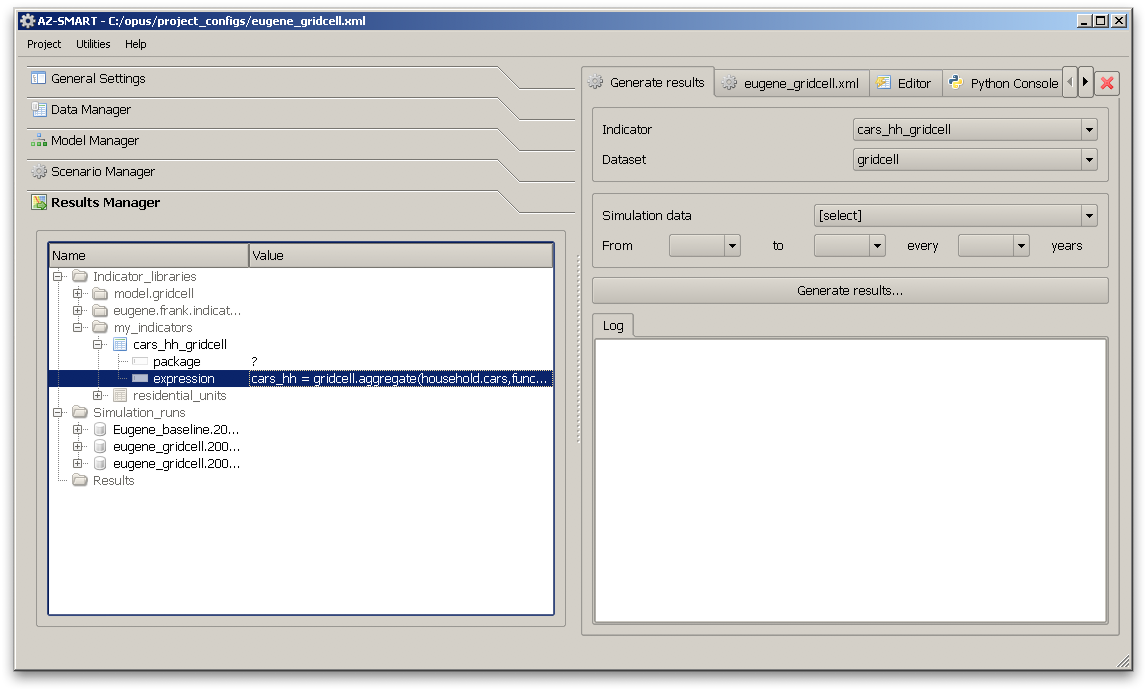
\includegraphics[scale=0.4]{graphics/indicator-cars-gridcell-1.png}
% \end{center}
% \caption{Generating the Average Cars per Household in a Gridcell}
% \label{fig:indicator-cars-gridcell-1}
% \end{figure}

\begin{figure}[htp]
\begin{center}
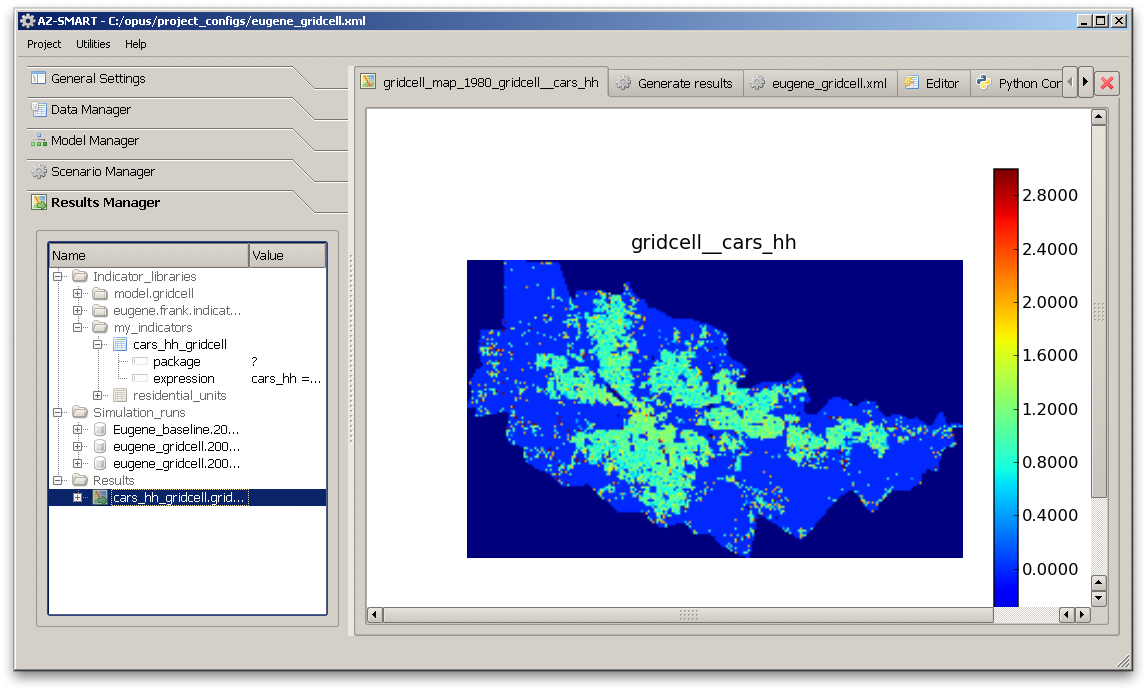
\includegraphics[scale=0.4]{graphics/indicator-cars-gridcell-2.png}
\end{center}
\caption{Generating the Average Cars per Household in a Gridcell}
\label{fig:indicator-cars-gridcell-2}
\end{figure}

In order to compute the second indicator, we will need to average the
number of cars per household at the zonal level as follows:

\code{cars\_per\_hh = zone.aggregate(household.cars, intermediates= [gridcell], function=mean)}

% T: this is actually not true, it works just fine
% The only remaining problem with this is that we cannot display zonal
% data using Matplotlib, which generates only raster image maps, meaning
% that it only supports displaying data assigned to gridcells.  Recalling
% the \verb#disaggregate# function in the expression language, we can
% just disaggregate the zonal average like this:
% 
% \code{cars\_per\_hh = gridcell.disaggregate(zone.aggregate(household.cars, intermediates= [gridcell], function=mean))}

To generate the third indicator of average household size we could use
a similar expression:

\code{persons\_per\_hh = zone.aggregate(household.persons, function=mean, intermediates = [gridcell])}

Now we use a compound expression, to sum the result of two variables,
and take the log of the result.  This is to produce the indicator as
shown below:

\code{ln\_emp\_pop=ln(urbansim.gridcell.population+urbansim.gridcell.number\_of\_jobs)}

Note that these are variables which can be found on the disk in
src/urbansim/gridcell.  The result of visualizing this indicator is
shown in Figure \ref{fig:indicator-ln-emp-pop}.

\begin{figure}[htp]
\begin{center}
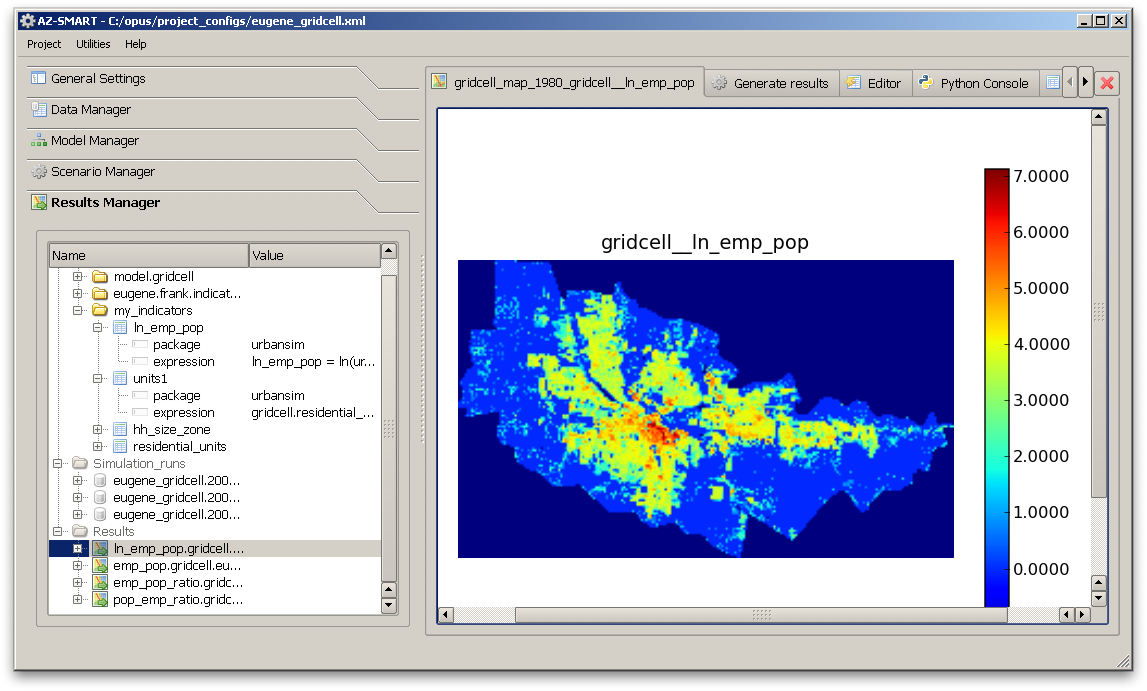
\includegraphics[scale=0.4]{graphics/indicator-ln-emp-pop.png}
\end{center}
\caption{Log of (Population + Employment) by Gridcell}
\label{fig:indicator-ln-emp-pop}
\end{figure}

% For the last indicators in the list to be done, we return to
% indicators that are already defined in a generic indicator library in
% the results manager.  To produce the population by zone indicator and
% visualize it as a table, use the following steps.  Right-click on the
% population indicators, and select \verb#Generate results with#.  In the
% form that is created on the right, select the pull-down menu labeled
% \verb#Dataset# and click on zone.  This is a generalized indicator that
% uses a simple mechanism to allow different levels of aggregation to be
% selected in this way, without the need to type in an expression as was
% done in the preceding examples.  Select a simulation result, and
% generate the indicator.  Then select the new indicator result
% containing the indicator values, right-click, and select \verb#View
% result as# and choose \verb#Table#.  This should generate a browsable
% table in the form window, as shown below in Figure
% \ref{fig:indicator-population-zone-table}.
% 
% \begin{figure}[htp]
% \begin{center}
% 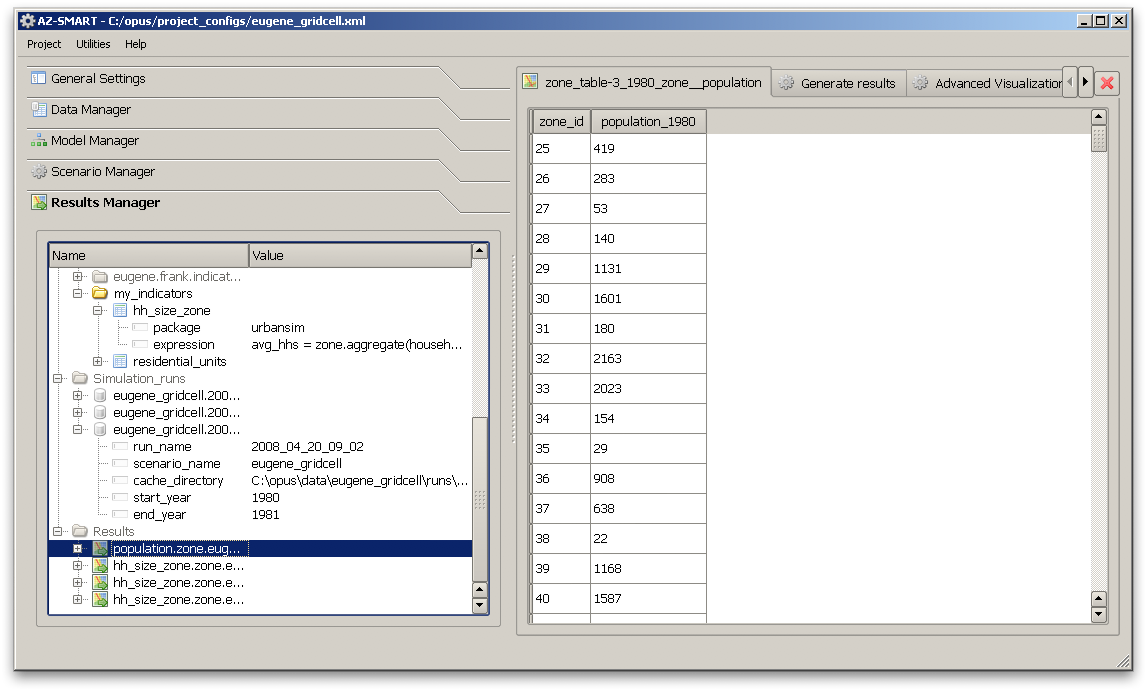
\includegraphics[scale=0.4]{graphics/indicator-population-zone-table.png}
% \end{center}
% \caption{Viewing the Population by Zone Indicator as a Table}
% \label{fig:indicator-population-zone-table}
% \end{figure}
% 
% Now that we have seen the integrated Matplotlib maps, you might want to
% know how to export an indicator to a more full-featured GIS system such
% as ArcGIS (a commercial package from Environmental Systems Research
% Institute), or PostGIS (an open source package built on the Postgres
% database).  The Results Manager is now able to export a table with one
% or more indicators to an ESRI Geodatabase for further analysis and
% visualization.  In the following example, we export the same indicator
% result shown above as a table, to an ESRI File-based Geodatabase. 
% Other Geodatabase formats are also supported.
% 
% If the population by zone table result is still available, right-click
% on the result in the tree on the left-hand side of the window, and
% select the \verb#View result as# and choose \verb#Advanced
% visualization#.  It will generate a form as shown in Figure
% \ref{fig:indicator-population-zone-export}.  We need to add the
% indicator we have generated to the set, in the upper portion of this
% form, and select the location of the ESRI geodatabase.  I am assuming
% that the geodatabase contains a \verb#Feature Class# corresponding to
% the table being exported. In this example, the table corresponds to the
% zone feature class.  Once the form is filled in, click on the
% \verb#Go!# button, to start the export process.  A message will be
% printed to the log to indicate the completion status of this export
% process.
% 
% \begin{figure}[htp]
% \begin{center}
% 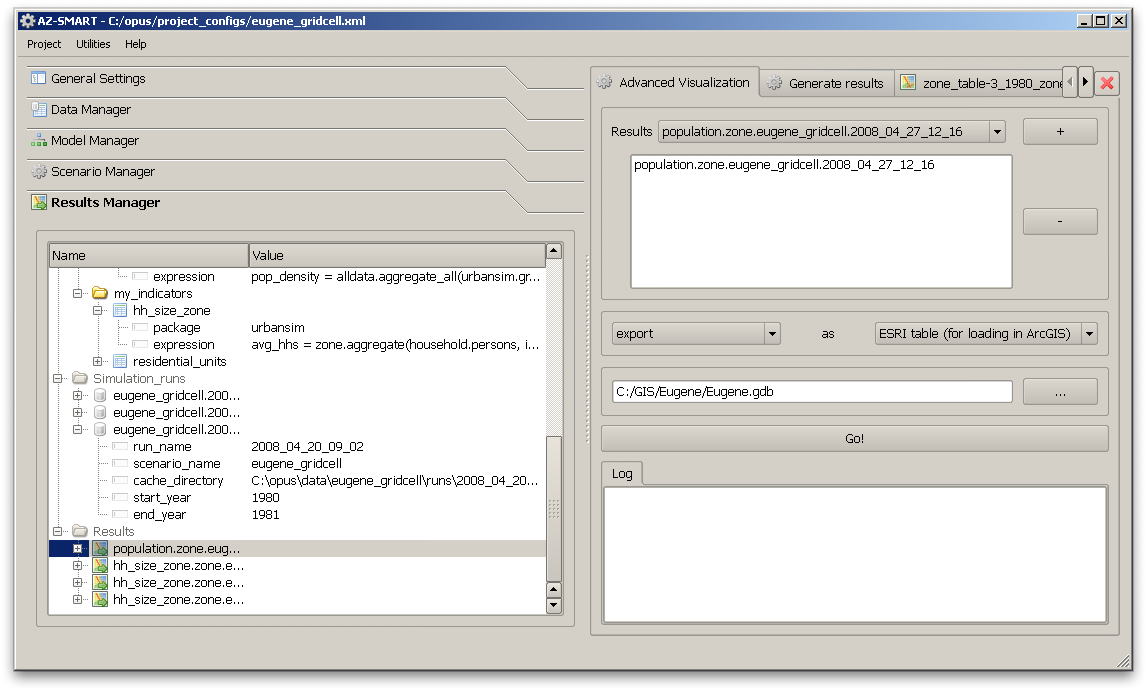
\includegraphics[scale=0.4]{graphics/indicator-population-zone-export.png}
% \end{center}
% \caption{Exporting the Population by Zone Indicator to an ESRI Geodatabase}
% \label{fig:indicator-population-zone-export}
% \end{figure}
% 
% Once the export is successfully completed, the geodatabase will contain
% a table that contains the indicator result, with a zone\_id and an
% ArcGIS \verb#OBJECTID*# that corresponds to the internal object ids in
% the feature class.  It is safe to join the indicator table result with
% the feature class using either the objectid or the zone\_id.  The map
% in Figure \ref{fig:indicator-population-zone-arcgis} shows the result
% of joining the feature class with the indicator table and generating a
% thematic map of the populaion by zone, using the zone.acres field to
% normalize the population, resulting in a map of population density per
% acre.
% 
% \begin{figure}[htp]
% \begin{center}
% 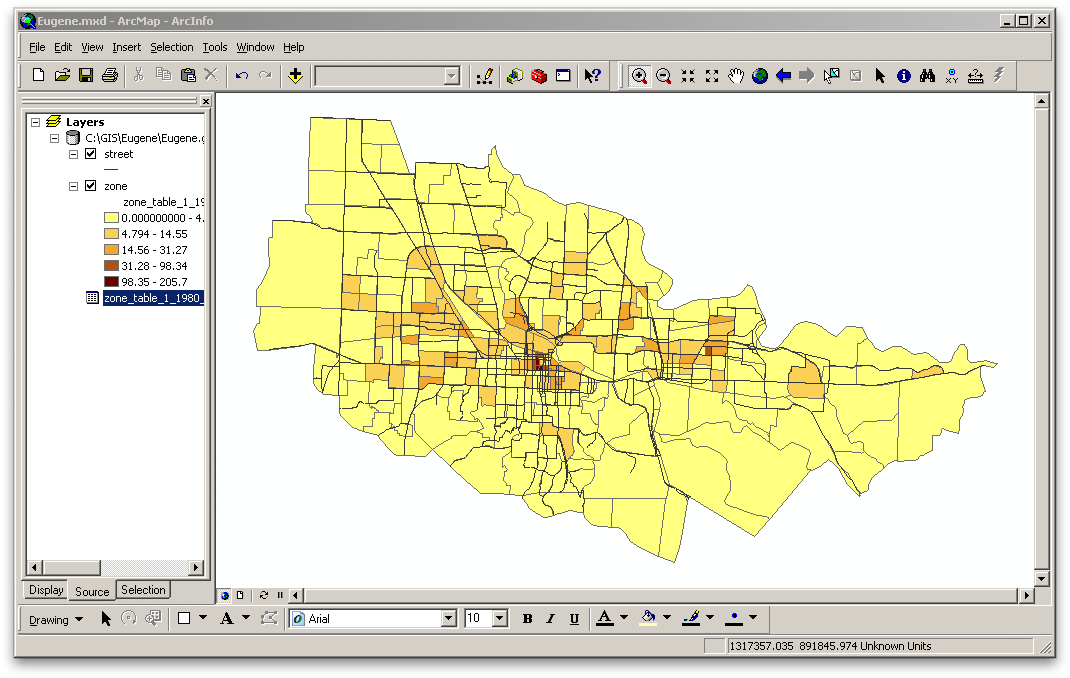
\includegraphics[scale=0.4]{graphics/indicator-population-zone-arcgis.png}
% \end{center}
% \caption{Mapping the Population by Zone Indicator in ESRI ArcMap}
% \label{fig:indicator-population-zone-arcgis}
% \end{figure}
